\section{Innledning og Teori}

    I analyse av RC-kretser er det et sentralt moment å beregne tidskonstanten $\tau$.
    Denne breskriver de karakteristikkene en gitt RC-krets innehar, som vil belyses i teorien.
    Det vil bli tydelig at verdien til $\tau$ er å finne både eksperimentelt ved analyse av spenning over tid, og uttrykt ved verdier på elektriske komponenter.

    Logiske kretser eksisterer i grenseland mellom ren matematikk og fysikk.
    Når en designer en krets på portnivå annses signaler vanligvis å være entydige binære verdier, men om man så analyserer kretsen på et lavere plan viser det seg at det ikke nødvendigvis er tilfellet.
    Dette forsøket tar for seg en sentral problemstilling ved det å designe logiske kretser 'for the real world'.

\subsection{Kondensatorer og RC kretser}

    \begin{itemize}
        \item[-] Kondensator: En kondensator er en passiv elektrisk komponent viss bruksområde er å lagre elektrisk ladning.
        Den består av to elektroder skilt med et dielektrisk materiale.
        Et dielektrisk materiale har elektrisk isolerende egenskaper og polariseres når det påvirkes av et elektrisk felt.
        Kondensatorer beskrives symbolsk ved likningen \ref{eq:farads}.
        \begin{equation}
            F = \frac{Q}{U}
            \label{eq:farads}
        \end{equation}
        I likning \ref{eq:farads} er $Q$ ladning målt i Coulomb, $U$ er spenning målt i Volt og $F$ er kapasitansen målt i Fahrrad.
        Fahrrad tilsvarer altså Coulomb/Volt.
        Kapasitansen beskriver mengden elektroner som må tilføres elektrodene for å danne en gitt spenning over dem.
        \item[-] RC-Krets: En enkel RC-krets består av en motstand og en kondensator koblet i serie se figur (3-1 ish).
        Spenning over kondensatoren i en slik krets kan beskrives ved \ref{eq:rc-oppladning} under oppladning og \ref{eq:rc-utladning} under utladning.
        \begin{equation}
            v_{C}(t) = V_{kilde} \cdot \left( 1 - e^{-\frac{t}{\tau}} \right)
            \label{eq:rc-oppladning}
        \end{equation}
        \begin{equation}
            v_{C}(t) = V_{kilde} \cdot e^{-\frac{t}{\tau}}
            \label{eq:rc-utladning}
        \end{equation}
        Begge er uttrykt ved tiden $t$ gitt i sekunder, og gjelder for $t \geq 0$.
        $\tau = R \cdot C$, $R$ er motstand målt i Ohm, og $C$ er kapasitans målt i Fahrrad.
        Se kapittel 7.2$^{~\ref{ECandDD}}$ for utledning av disse formlene.
    \end{itemize}

\subsection{Transistorer}

    \begin{itemize}
        \item[-] PMOS-, og NMOS-transistor: De mest grunnleggende byggeklossene i logiske kretser er disse to formene for transistor, som begge fungerer som brytere.
        PMOS slipper signaler gjennom ved input: lav, og blokkerer dem ved input: høy.
        NMOS fungerer på samme måte, men invertert.
        Se figur~\ref{fig:pnmos_transistors} Ved bruk av disse kan man konstruere alle logiske porter.
        \item[-] NAND port: En to-inngangs NAND port er en logisk port som tar to binære input signaler og utfører funksjonene NOT og AND på dem for å produsere ett output signal.
        Se figur~\ref{fig:tt_nand} for sannhetstabellen til NAND porten.
        Se figur~\ref{fig:NAND_transistorlevel} for oppbyggingen av en NAND port med bruk av PMOS-, og NMOS-transistorer.
        \item[-] Kombinatorisk CMOS-logikk: En CMOS krets består av en eller flere logiske porter bygget på PMOS-, og NMOS-transistorer.
    \end{itemize}

    \begin{figure}[!htb]
        \centering
        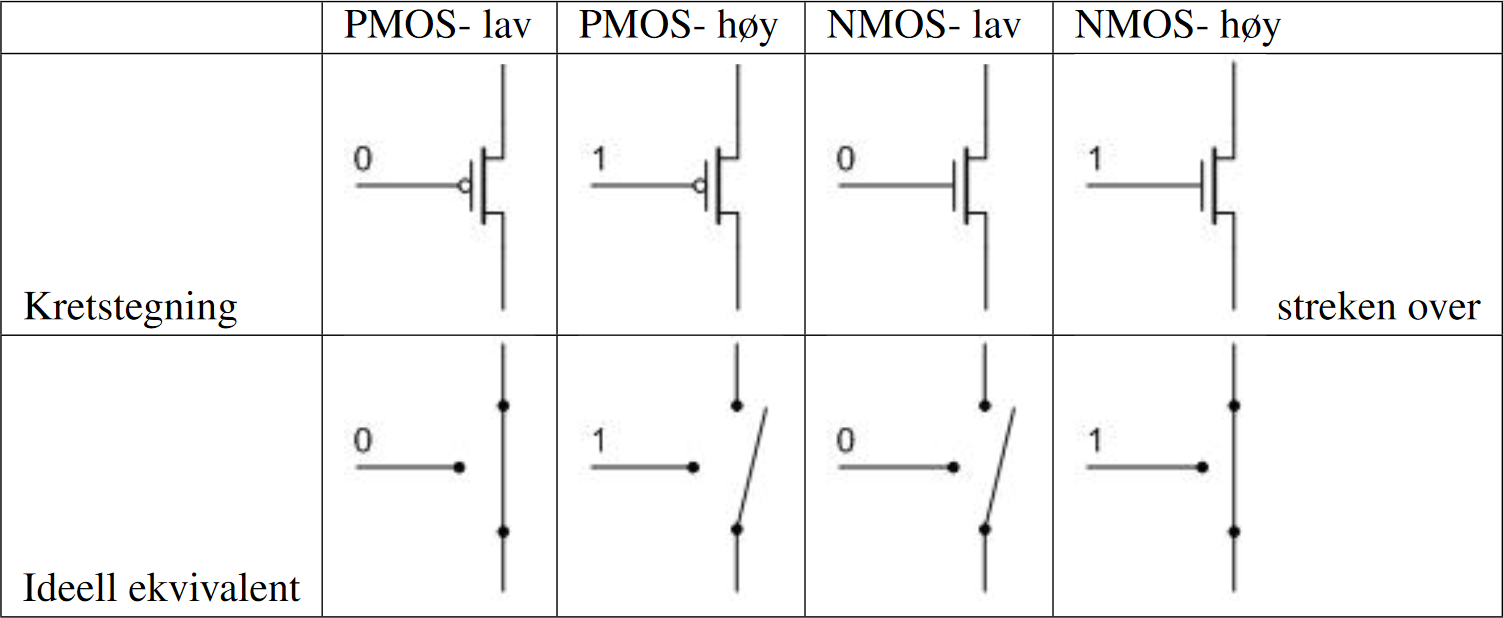
\includegraphics[height=4cm]{figurer/PNMOS.png}
        \caption{PMOS og NMOS- transistor med deres ideelle ekvivalenter for åpen og lukketkanal.}
        \label{fig:pnmos_transistors}
        ~\cite{labhefte}
    \end{figure}

    \begin{figure}[!htb]
        \centering
        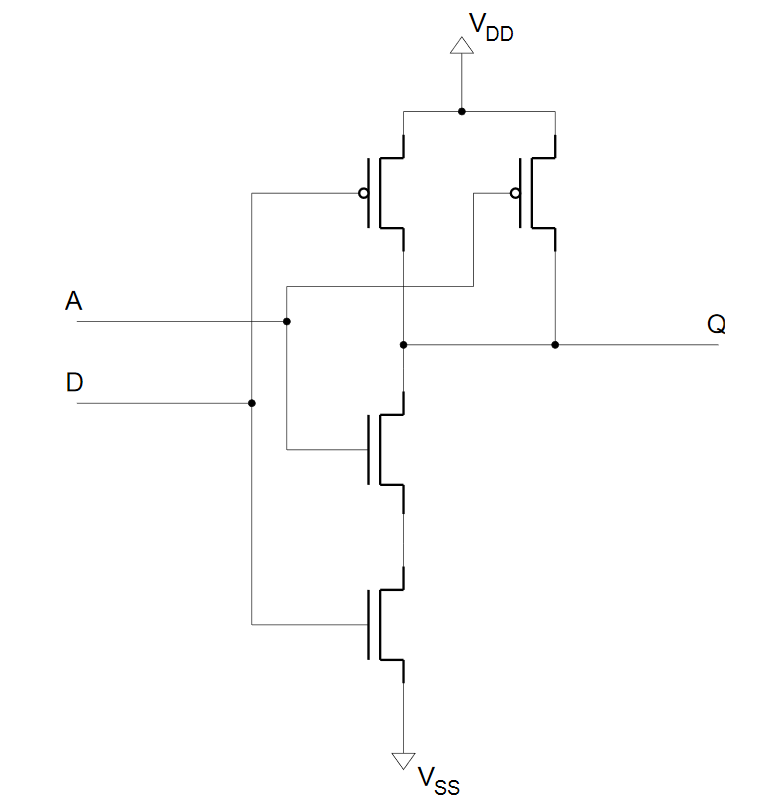
\includegraphics[height=8cm]{figurer/NAND_transistorlevel.png}
        \caption{NAND port på transistornivå.}
        \label{fig:NAND_transistorlevel}
        ~\cite{labhefte}
    \end{figure}

    \begin{figure}[!htb]
        \centering
        \begin{tabular}{|c|c|c|}
            \hline
            \textbf{A} & \textbf{B} & \textbf{A NAND B} \\ \hline
            0 & 0 & 1 \\
            0 & 1 & 1 \\
            1 & 0 & 1 \\
            1 & 1 & 0 \\ \hline
        \end{tabular}
        \caption{Sannhetstabell for NAND port}
        \label{fig:tt_nand}
    \end{figure}